%\documentclass[a4paper,12pt]{article}
\documentclass{llncs}
%\documentclass[12pt]{paper}
%\documentclass[a4paper,twoside,twocolumn]{article}
\usepackage{authblk}

\usepackage[utf8x]{inputenc}
\usepackage[english]{babel}
\usepackage{subfigure}
\usepackage{float}
\usepackage{placeins}
\usepackage{graphicx}
\usepackage{array}
%\usepackage[]{algorithm2e}
\usepackage{setspace}
\usepackage{xspace}
\usepackage{cite}
\usepackage[show]{notes}
%\onehalfspace % interlinea 1.5
%\doublespace % interlinea 2
%\usepackage[stdsize,thm]{botex}
%\usepackage{amsthm}
%\theoremstyle{plain}
%\newtheorem{thm}{Theorem}[chapter]
%\newtheorem{cor}[thm]{Corollary}
%\newtheorem{lem}[thm]{Lemma}
%\newtheorem{prop}[thm]{Proposition}
%\theoremstyle{definition}
%\newtheorem{defn}{Definition}[chapter]
\usepackage{hyperref}
%\usepackage[bookmarksopen,bookmarksdepth=2,breaklinks=true]{hyperref}

\newcommand{\AlgFont}[1]{\textbf{#1}}

\newcommand{\GB}{\AlgFont{GB}\xsp
ace}
\newcommand{\ADA}{\AlgFont{ADA}\xspace}
\newcommand{\BAG}{\AlgFont{BAG}\xspace}
\newcommand{\DT}{\AlgFont{DT}\xspace}
\newcommand{\RF}{\AlgFont{RF}\xspace}
\newcommand{\NAIVE}{\AlgFont{NAIVE}\xspace}
\newcommand{\MNB}{\AlgFont{MNB}\xspace}
\newcommand{\LOG}{\AlgFont{LOG}\xspace}
\newcommand{\COMB}{\AlgFont{COMB}\xspace}

\newcommand{\MeasuresFont}[1]{\textbf{#1}}

\newcommand{\TP}{\MeasuresFont{TP}}
\newcommand{\FP}{\MeasuresFont{FP}}
\newcommand{\TN}{\MeasuresFont{TN}}
\newcommand{\FN}{\MeasuresFont{FN}}
\newcommand{\Precision}{\MeasuresFont{Pr}}
\newcommand{\Recall}{\MeasuresFont{Re}}
\newcommand{\FOne}{\MeasuresFont{F1}}
\newcommand{\TypeOne}{\MeasuresFont{Type-I}}
\newcommand{\TypeTwo}{\MeasuresFont{Type-II}}
\newcommand{\Bacc}{\MeasuresFont{BACC}}



\title{Firms Default Prediction with Machine Learning}
\author{Tesi Aliaj\inst{1} \and Aris
  Anagnostopoulos\inst{1}\thanks{Partially supported by ERC Advanced
    Grant  788893 AMDROMA ``Algorithmic and Mechanism Design Research in Online Markets.''} \and Stefano
  Piersanti\inst{1}\inst{2}}

\institute{
Sapienza University of Rome, Italy.
  \email{tess.aliaj@gmail.com, aris@diag.brown.edu, piersanti@diag.uniroma1.it}
\and Bank of Italy}



\begin{document}

\maketitle


\begin{abstract}



Finding a model to predict the default risk of a firm is a well-known topic over the financial and data science community. Many modern approaches triumph in finding well-performing models to forecast it. Those models often act like a black-box and don't give to financial institutions the fundamental explanations they need for their choices.
This paper aims to find a robust predictive model using a tree-based machine learning algorithm which flanked by a game-theoretic approach can provide sound explanations of the output of the model. Our study uses in combination, for the first time, two large and sparse datasets of credit data from the Italian Central Credit Register of Bank of Italy and from ECB AnaCredit survey that contain information on all Italian companies' past behaviour towards the entire Italian banking system. 
In the end, we show how our model outperforms the current predictions made by institutions and at the same time, provides insights on the reasons that lead to a particular outcome.




%In line with the results of \cite{altman-bankruptcy-17} we find that
%bagging, boosting, and random forest models outperform the others
%techniques, in particular logistic regression. In this sense also our
%research related to default prediction adds to the discussion of the
%continuing debate about superiority of computational methods over
%statistical techniques.


\end{abstract}


%\chapter{Abstract}

\section{Introduction}
\label{sec:intro}

Bankruptcy prediction of a company is, not surprisingly, a topic that
has attreacted a lot of research in the past decades by multiple
disciplines~\cite{altman-bankruptcy-17,kumar-review-07,chen-bankruptcy-11,lee-bankruptcy-13,erdogan-bankruptcy-13,cho-bankruptcy-10,wang-bankruptcy-11,Altman-8,Ohlson-9,Begley-10,Lee-10a,Fernandez-11,Odom-13,Atiya-15,Wang-16}.
Probably the main importance of such research is in bank lending.
Banks need to predict the possibility of default of a potential
counterparty before they extend a loan.
An effective predictive system can lead to a sounder and profitable
lending decisions leading to significant savings for the
banks and the companies and, most importantly, to a stable financial
banking system.
A stable and effective banking system is crucial for
financial stability and economic recovery as well highlighted by the
recent global financial crisis and European debt crisis.
%The magnitude of bankruptcy costs is a critical issue in terms of
%capital structure theories.
\notes[Aris]{It would be good if we can put a number (and a citation) on
the cost of bankrupt companies on the banking system.}

\notes[ste]{"But in Italy where families and businesses are financed mainly by credit, the wave of corporate bankruptcies and the sharp rise in unemployment have been reflected in an increase in bad debts, and consequently in a worsening of the banks' financial situation.
The growth of the new deteriorated bank loans and the slowness of the judicial recovery procedures have determined a rapid increase in the stock of these assets, which in 2015 reached a peak of 200 billion, equal to 11 percent of total loans."  (Fabio Panetta, Deputy Governor of the Bank of Italy - Rome - Camera dei Deputati - May 2018)}

Of course, despite the pletora of studies, predictiong the failure of a
company is a hard task, as demonstrated by the 
enormous increase in large corporate failures in
the last decades.

%
%
%It has also crucial importance to predict
%probability of bankruptcy in the assessment of companies’
%creditworthiness.
%
% has revealed the importance of bankruptcy prediction
%and enforced to improve new techniques.
%
%The keystone studies of
%bankruptcy literature, different findings and views regarding
%problematic issues of bankruptcy are presented in several studies.
%
%The
%inconclusive results indicate that bankruptcy prediction will remain an
%attractive field for all parties of financial world.
%Therefore, the accurate prediction of bankruptcy remains in any case a
%very important problem in financial and banking management. Basically,
%it is a binary classification problem, which includes two classes
%namely \textit{bankrupt} and \textit{non-bankrupt}. 

\notes[Aris]{Stefano, please check the paragraph below.}
\notes[ste]{OK good}

Most related research has focused on \emph{bankruptcy} prediction, which
takes place when the company officially has the status of being unable
to pay its debts (see Section~\ref{sec:problem}). However, companies
often signal much earlier their financial problems towards the banking
system by going in \emph{default}. Informally speaking, a company enters
into a default state if it has failed to meet its requirement to repay
its loans to the banks (see Section~\ref{sec:problem}). Entering into a
default state is a strong signal of a company's failure: typically banks
do not finance a company into such a state and it is correlated with
future bankruptcy.

In this paper we use historic data for predicting whether a company will
enter in default. We base our analysis on two sets of data. First, we
use historic information from \emph{all the loans} obtained by \emph{almost all
the companies} based in Italy (totaling to around $800K$ companies).
This information includes information on the companies credit dynamics in the past
years, as well as past information on relations with banks and on values of protections related to loans
\notes[Aris]{what should we write here?}
\notes[ste]{I add some concepts}
Second, we combine these data with the balance sheets of $300K$
of these companies (the rest of them are not obliged to produce balance
sheets). We apply multiple machine-learning techniques, showing that the
future default status can be predected with reasonable accuracy.
Note that the dimensions and the information in our dataset exceeds
significantly those of past work, allowing to obtain a very accurate
picture of the possibility to predict over various economic sectors.


\paragraph{Contributions.} To summarize the contributions of our paper
\begin{enumerate}
\item We analyze a vary large dataset ($800K$ companies) with granular
data (every quarter) on the performance of each company over a period of
10 year. 
\item We use these data to predict whether a company will default in the
next year.
\notes[Aris]{That's what we do, right? We go back 5 quarters, correct?
Have we tried to use data from the previous year? That is, use data from
2017 to predict what will happen in 2019.}
\notes[ste]{Yes the results are obtained using the previous 5 quarters. In particular we try to forecast default from dec 2014 to dec 2015 (for firms that are OK in dec 2014) using data from sep 2013 to dec 2014. To use more data (I've tried actually up to 5 years if I remember well) seems not improve signiificant the performance}
\item We combine our data with data available from company balance
sheets, showing that we can improve further the accuracy of predictions.
\end{enumerate}

\paragraph{Roadmap.} In Section~\ref{sec:related} we present some related
work. In Section~\ref{sec:problem} we provide definitions and we
describe the problem that we solve. In Section~\ref{sec:approach} we
describe our datasets and the techniques that we use and in
Section~\ref{sec:experiments} we present our results. We conclude in
Section~\ref{sec:conclusion}.

%
%\subsection{Bankruptcy and firms default prediction problem}
%
%Bankruptcy and firms default prediction problem are two key issues
%strongly connected.
%
%Corporate loan default prediction has become an
%increasingly important problem for financial institutions due to the
%advanced and recent financial crisis.
%
%In this article we will examine in
%particular this issue choosing a very simple approach applied to an
%Italian database containing information on credit data.
%
%To get an idea about the potential impact of the loan default prediction
%problem, we note that the volume of outstanding debt to corporations in
%the Euro area is about 5 trillion of euro.
%
%The \textit{“Non performing
%loans”} (NPL) are about 500 billions and they recently increased
%considerably as a result of the financial crisis and business
%failures.
%
%An improvement in loan default prediction accuracy of just a
%few percentage points can lead to savings of tens of billions of
%dollars.
%
%In this article we focus only on the corporate loan default prediction
%problem and we do not address prediction regarding the consumer loans
%(i.e. loan to households, for example for house purchase).
%
%Several recent and advanced techniques for predicting bankruptcy have
%been developed \cite{kumar-review-07} \cite{wang-bankruptcy-11} over the
%years.
%
%Statistical and Machine Learning techniques are the two broad
%categories used to predict bankruptcy \cite{chen-bankruptcy-11}
%\cite{kirkos-fraudulent-07}.
%
%Statistical techniques include linear discriminant analysis (LDA),
%multi-discriminant analysis (MDA) \cite{lee-bankruptcy-13}, logistic
%regression (LR), etc, while Machine learning techniques (ML) include
%well-known algorithms such as Artificial neural networks (ANN), SVM
%\cite{erdogan-bankruptcy-13}, Decision trees \cite{cho-bankruptcy-10}
%and Random Forest.
%
%\begin{figure}[H]
%
\includegraphics[width=160mm, height=60mm]{figs/CFig1.png}
%\caption{Principal techniques used to predict bankruptcy of the firms.}
%\end{figure}
%
%There are two main approaches to loan default prediction problem.
%
%The
%first approach, the structural approach, is based on modeling the
%underlying dynamics of interest rates and firm characteristics and
%deriving the default probability based on these dynamics.
%
%The second
%approach is the empirical or the statistical approach. Instead of
%modeling the relationship of default with the characteristics of a firm,
%this relationship is learned from the data.
%
%The focus of this article is on the empirical approach, especially the
%use of Decision Tree, Random Forest and others well-known Machine
%Learning techniques.
%
%Figure 1 shows the principal techniques used to address the bankruptcy
%prediction problem.
%
%
%
%
%
%
%This article is structured as follows: 
%section II contains a literature review, which briefly discusses the
%various statistical and machine   learning techniques that have been
%proposed by various researchers. Section III describes the prediction
%problem, the dataset and the techniques used for the prediction
%exercise. Section IV presents the experimental results. Finally, Section
%V concludes the paper.




\section{Related Work}
\label{sec:related}

%\subsection{A review of related work}
There has been an enormous amount of work on bankruptcy prediction. 
In order to give a flavor of how the literature that concerns bankruptcy prediction models has evolved, we briefly review the most influential previous studies below.


\subsection{Early approaches}

Initially, scholars focused on making a linear distinction among healthy
companies and the ones that will eventually default. Among the most
influencing pioneers in this field we can distinguish
Altman~\cite{Altman-8} and Ohlson \cite{Ohlson-9}, both of whom made a
traditional probabilistic econometric analysis. Altman, essentially
defined a score, the $Z$ discriminant score, which depends on several
financial ratios (working capital/total assets, retained earnings/total
assets, etc.) to asses the financial condition of a company.
Ohlson on the other side, is using a linear
regression (LR) logit model that estimates the probability of failure of
a company and identifies four main factors that affect that probability: the company’s size, its financial structure, its financial performance and its liquidity.

Some papers criticize these methods as unable to classify companies as viable or nonviable~\cite{Begley-10}. However, both
approaches are used, in the majority of the literature, as a benchmark
to evaluate more sophisticated methods.
Those sophisticated methods are the machine learning techniques which are the focus of this paper. Below, we provide a glimpse at the evolution of different techniques and at the comparison among them in the literature.

Since these early works there has been a large number of works based on machine-learning techniques \cite{lin-12, devi-18, nanni-09}.
The most successful have been based on 
decision trees \cite{Lee-10a, Zhou-10b, Gepp-10b, Martinelli-12} and neural networks
\cite{Fernandez-11, Odom-13, Boritz-14,Atiya-15,Wang-16}. Typically, all
these works use different datasets and different sets of features, depending on the dataset.

One of the first applications of the neural network methods for bankruptcy prediction, is that of Odom and Sharda \cite{Odom-13}. They compared a three perceptron network against a method that was the "rule" until then: the multivariate discriminant analysis using the Altman ratios explained above, and it proved to be more robust in terms of accuracy. Boritz et al \cite{Boritz-14} uses two different techniques to train a neural network: back-propagation and Optimal Estimation Theory (OET), and compares them to more traditional methods such as discriminant analysis, probit and logit, as well as against benchmarks provided by directly applying the bankruptcy prediction models developed by Altman and Ohlson which were previously explained. They find no superiority for neural networks; instead the performance of each technique can be improved based on the relative size of the test and train set on the nature and number of imports etc. Nevertheless, it should be mentioned that they test only one architecture of a neural network.
Atiya \cite{Atiya-15} suggests the inclusion of features extracted from equity markets because as he states “tend to be highly predictive, not only of the health of a firm, but also of the health of the economy, which in turn affects the creditworthiness of the firm”, with a resulting improvement in accuracy of around four percentage points. What we can grasp from this retrospective look of previous experiments is that, that machine learning techniques probably will perform better in our bankruptcy prediction problem, but regarding the comparison among decision trees and NNs the feelings are mixed. We cannot, though, state with certainty ex-ante which of them will be superior.

There exists a wide range of classification methods included in the category of decision trees. Lee \cite{lee-bankruptcy-13} by making a comparison of three of them using a dataset of Taiwan listed electronic companies concludes that the most efficients (in terms of accuracy) is the Generic Programming decision tree classifier which represents “a technique that applies the Darwinian theory of evolution to develop efficient computer programs (Koza ,1992)”.
Zhou and Wang \cite{Zhou-10b} on the other side, starting from the traditional random forest, propose the assignment of weights to each of the decision trees created, which are retrieved from each tree’s past performance (out-of-bag errors in training method). They show that this modification improves the performance of the algorithm in terms of overall accuracy as well as the accuracy of their balanced dataset. Gepp and Kumar \cite{Gepp-10b} turn their attention to another method, the Cox survival analysis, and compare it to the CART decision tree classifier and conclude that the former is the best one-year bankruptcy predictor, while the latter outperformed in the three-year prediction. Fernandez and Olmeda \cite{Fernandez-11} compared NN with MDA, LR, MARS and C4.5 (two well-known methods that are based on the CART decision tree algorithm) on Spanish banks and showed that NN resulted in a higher accuracy. Martinelli et al. \cite{Martinelli-12} by doing a very similar analysis on a database of Brazilian firms showed that the C4.5 algorithm is the one that outperforms the other methods.

\subsection{More recent works}

Chakraborty and Joseph (2017) train a set of models to predict distress in financial institutions based on balance sheet items, finding that ML approaches generally outperform statistical models based on logistic regression. Specifically, the RDF model allows for a marked increase in discriminatory power of about 10 percentage points in terms of the Area under the Receiver Operating Characteristic (AuROC) compared with the logit model.
Using data on US household default on mortgages, Fuster et al. (2018) find that the RDF model generates more accurate predictions than the logit model, although the improvement is minimal and accounts for about 1.2 percentage points of AuROC. The authors argue that most of these gains result from the sophisticated functional form of the RDF model, which captures the complex relationships connecting different variables to default outcomes with greater discriminatory power. 
Albanesi and Vamossy (2019) develop a model to predict consumer default based on deep learning (i.e. a combination of forecasts from deep neural network and gradient boosting) in environments with high-dimensional data (over 200 variables).
In a recent very important study, Barboza et al. \cite{altman-bankruptcy-17} compare such techniques with support vector machines and ensemble methods showing that ensemble methods and random forests perform the best.
Recently, Andini et al. ~\cite{andini-19} have used data from Italian Central Credit Register to assess the creditworthiness of companies in order to propose an improvement in the effectiveness of the assignment policies of the public guarantee programs.
The majority of the cited works typically try to predict bankruptcy of a company. Our goal is to predict both bankruptcy and bank default, after  explored the related connections between the two critical situations. Furthermore, most of these papers use balance sheet data (which are public). Our dataset contains a very granular information of a very large set of companies on the past behavior of loan repayment. In particular, we use two different important sources of credit information: the Italian Central Credit Register and, for the fist time given the novelty, the Italian component of AnaCredit, that is a very recent European credit dataset. We combine credit data with balance sheet data in order to show that the combination of the two source of information improve the prediction performances.
To our knowledge, our dataset is one of the most
extensive dataset used in the literature.
But the crucial point we wanted to address is that of trying to explain the predictions, investigating through the use of SHAP, the crucial factors that could explain the failures of companies.









\input{problem.tex}
\section{Data and Methods}
\label{sec:approach}

\subsection{Dataset Description}

We have used the following two datasets. The first and most important in our work is composed of information on loans and the credit of a large sample of Italian companies. The second reports balance sheet data of a large sub-sample of medium-large Italian companies.


\paragraph{Credit data.} 


It consists of a very large and high granular dataset of credit
information about Italian companies belonging to the Italian Central
Credit Register.
It is an information system on the debt
of the customers of the banks and financial companies supervised by the
Bank of Italy. Bank of Italy collects information on customers'
borrowings from the intermediaries and notifies them of the risk
position of each customer vis-à-vis the banking system.
By means of the Central Credit Register the Bank of Italy provides
intermediaries with a service intended to improve the quality of the
lending of the credit system and ultimately to enhance its stability.
The intermediaries report to the Bank of Italy on a monthly basis the
total amount of credit due from their customers: data information about
loans of 30,000 euro or more and non-performing loans of any amount.

Italian Central Credit Register has three main goals: a)
improve the process of assessing customer creditworthiness; b) to
raise the quality of credit granted by intermediaries; c) strengthen
the financial stability of the credit system. 




The crucial feature of this database is the high granularity of credit
information. To the best of our knowledge, Machine Learning techniques
have not yet been applied for the analysis of these database.
We used a overall credit dataset containing over 800,000 rows. Each row contain credit
data related to a single firm. For each firm the dataset contains about
20 different attributs; the most important are shown in the following
Table. We considered information on the dynamics
of credit to firm with quarterly frequency. The objective of the work is
to predict whether a company that at the time T was not in default
status in the following year will be classified in default. The complete
dataset used to make the predictions consists of credit information over
a period of five years from 2009 to 2014.
Central Credit Register data are not public.



\begin{figure}[H]
\flushleft
%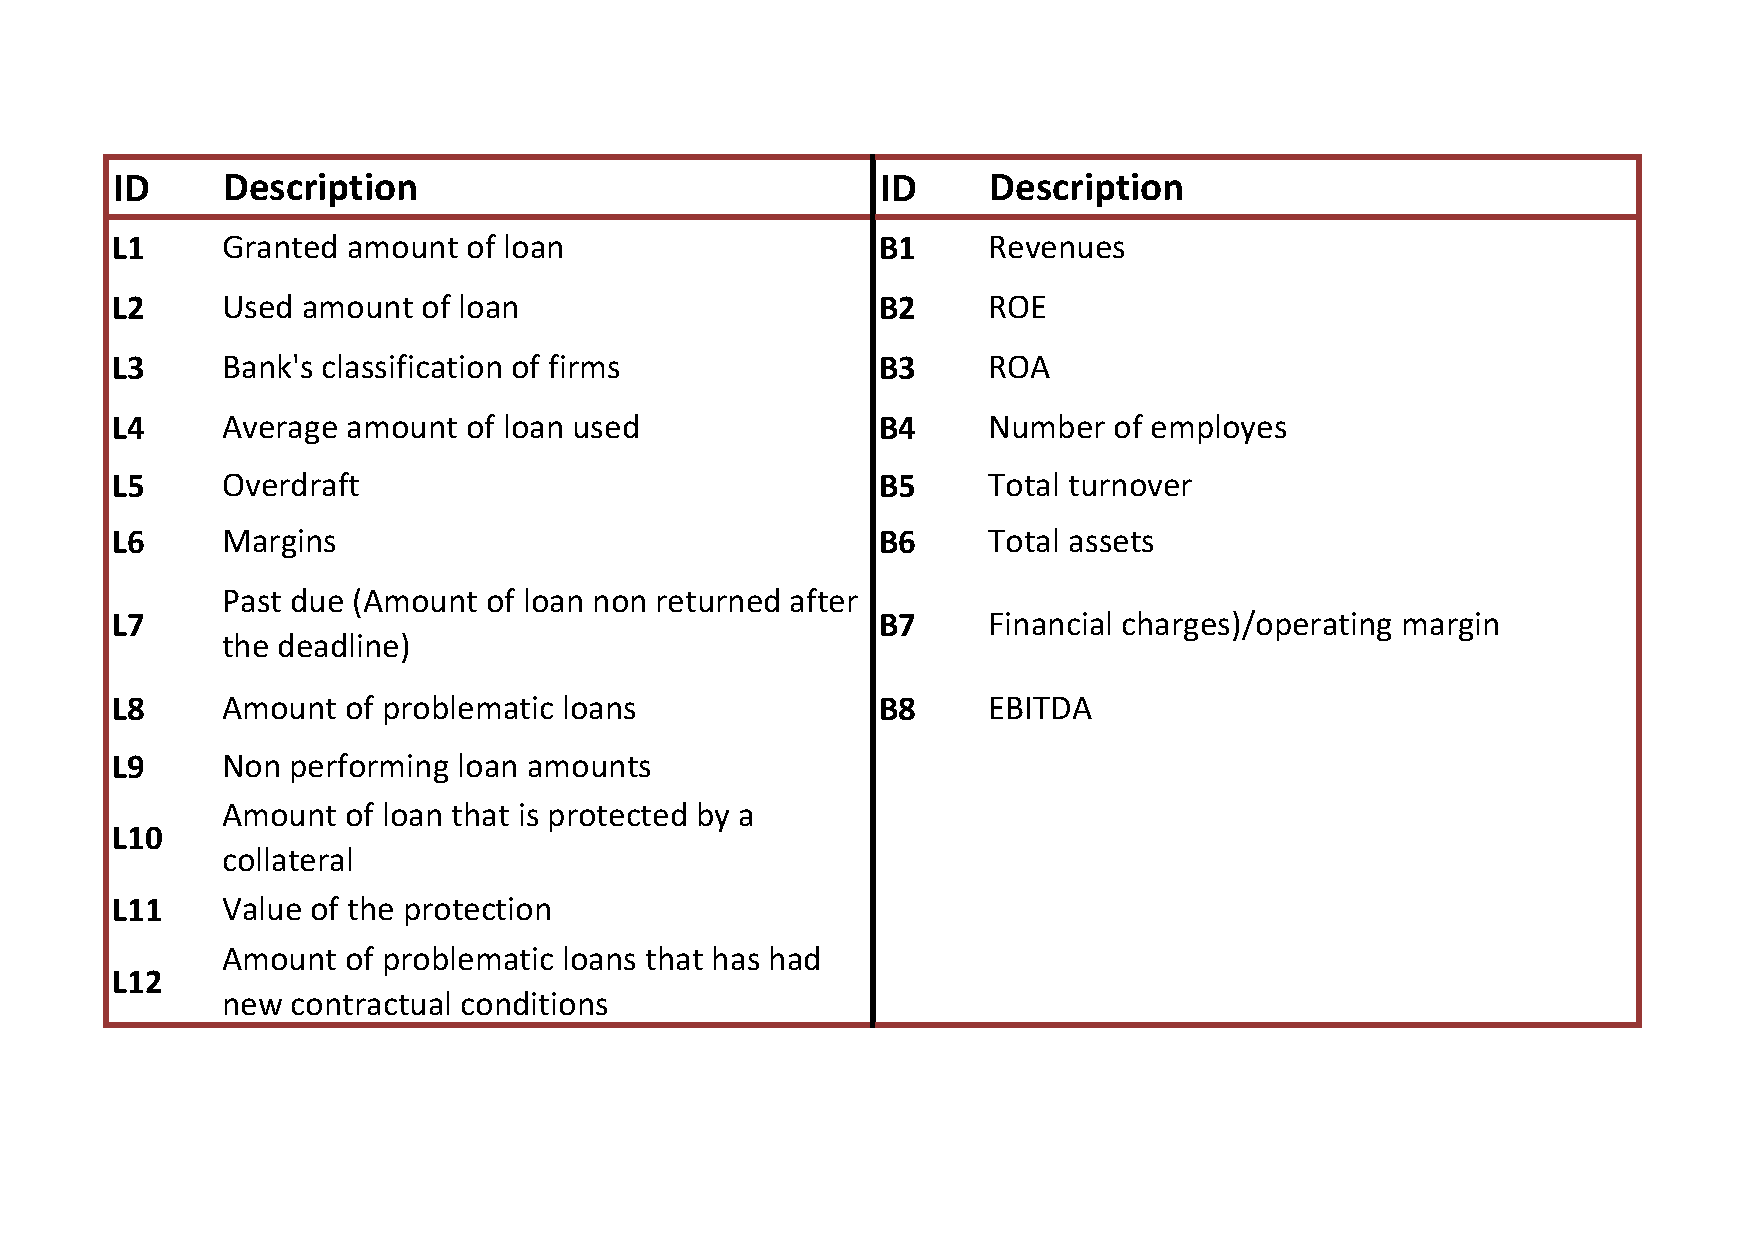
\includegraphics[width=180mm, height=80mm]{figs/Table_dataset.pdf}
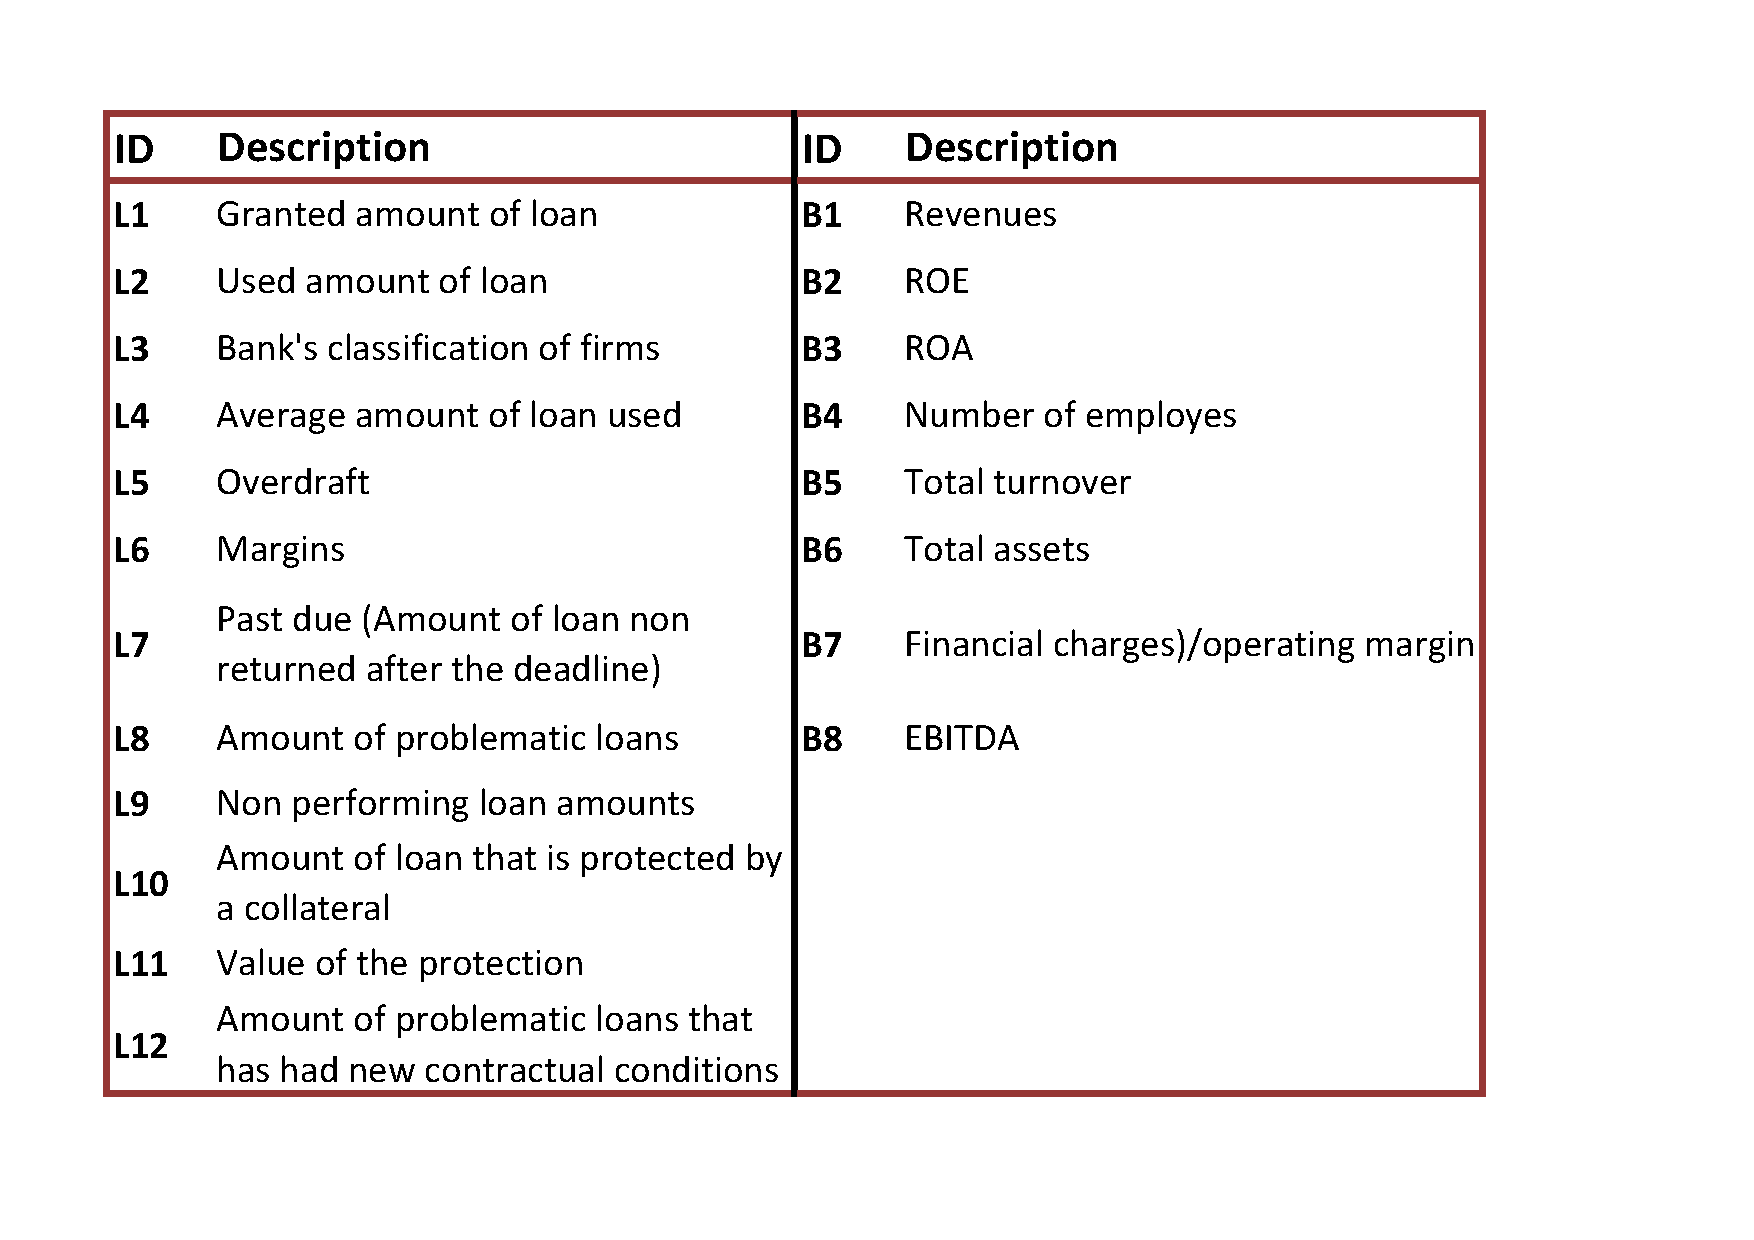
\includegraphics[width=180mm, height=80mm]{figs/Cdataset.pdf}
\caption{Loan dataset (L) and Balance sheet dataset (B): main
attributes. Loans data are quarterly from 2009 to 2014;
Balance sheet data have annual frequency from 2006 to 2014}
\end{figure}


\paragraph{The Balance sheet dataset.}



With the aim of improving the forecasts of the default status of Italian
firms, we have also performed some classification attempts  by
integrating credit information with some balance sheet indicator for Italian
companies. In particular, we used a set of firms balance sheet
indicators from the CEBI dataset: some important indicators are used
that are very similar to those used by Altman
\cite{altman-bankruptcy-17} also  in his famous Z-score. Among the
fundamental ones are those regarding the profitability of companies, as
in the case of ROE and ROA. The balance sheet dataset contains data
related to about 300,000 Italian firms; these are generally medium and
large companies. For each firms we used a set of eight indicators shown
in the Table. Balance sheet data are public data.\\
The three hundred thousand companies for which balance sheet data are available constitute a sub-sample of those belonging to the loan dataset. Therefore the dataset that uses both information on loans and balance sheet info is made up of about 300,000 companies.








\input{experiments.tex}
\section{Conclusion}
\label{sec:conclusion}

Business-failure prediction is a very important topic of study for economic analysis and the regular functioning of the financial system. Moreover the importance of this issue has greatly increased following the recent financial crisis. 
Furthermore, we can certainly consider that the current global crisis caused by Covid-19 will lead to a significant increase in business failures by amplifying the relevance of a good ability to analyze and predict phenomena.

There have been many recent studies that have tried to predict the failure of companies using various machine-learning techniques.
In our study, we used for the first time credit information from the ItalianCentral Credit Register and from ECB AnaCredit survey to predict the banking default of Italian companies, using Machine Learning and other well-known statistical techniques.
We analyzed a very large dataset containing information about almost all the loans of all the Italian companies. Our first findings is that, both in the case of bankruptcy prediction and banks default prediction, machine-learning approaches are able to outperform significantly simpler statistical approaches.


In fact, our results confirm the best performance of Machine learning classifier respect to other well-known statistical methods. In addition we show that some recent types of boosting classifiers obtain the best results. 
 \\
 Furthemore, in this paper we explored the differences and links between corporate failures and bank defaults. We focus our analysis both on bankruptcy, a well-known issue in literature, and on the bank default, which in many cases anticipates the failure of a company. At the same time it represents an important sign of vulnerability as typically a company in bank default is unable to repay its debts.
 \\
 We use Central Credit Register data in combination with balance sheet data in order to predict both bankruptcy and adjusted default. We show that this combination of data can lead to robust performance in prediction. 
 In fact, using information on past loan data is crucial, but the additional use of balance-sheet data can improve classication even further. We show that the combined use of loan data with balanced-sheet data leads to nice performance for predicting default. We also show that using loan data in the prediction of bankruptcy (where, typically, only balance-sheet data are being used) can play an important role.
 The forecast performances obtained are very similar, but a relevant point seems to be that balance sheet data seems to be more suitable for predicting bankruptcies, while the loan data helps to predict bank defaults much better. We corroborate this conjecture also in terms of expainability of the prediction results.
 
 In addition we use, for the first time given the novelty of this source of data, also information data from ECB AnaCredit survey, recently started under the coordination of ECB, in order to improve adjusted default prediction in the more recent years.  We try to exploit the predictive capacity of our credit information by using BORUTA, a  feature selection technique that seems to work very well in our case.
 
 This approach seems to improve prediction performance allowing to obtain remarkable results, with an AuROC of 0.93, even in comparison to the most relevant literature on the subject.
 \\

 Moreover, a relevant point of our work concerns the attempt to explain default predictions; this theme is indeed very relevant for the practical use of forecasting techniques. To this end we used SHAP, a modern method to extract the importance of features in the forecast, showing a robust dependence of our predictions on a series of information that have an important economic significance.
 For example, as easily understood, probability of default (PD) assessed by the banking system play a significant role in a bank default prediction. But a  comparison exercise with the default prediction based only on PD used by banks shows that predictions with Machine learning provide a very significant gain in performance.
 \\
 \\
 Nevertheless, prediction remains an extremely hard problem in this field with very unbalanced dataset. Yet, even slight improvement in the performance, can lead to savings of multiple hundreds of thousands of euros for the banking system. Thus our goal is to improve classification even further by combining our approaches with further techniques, such as neural-network based ones. Some preliminary results in which we use only neural networks are encouraging, even though are worse than the results we report here.
 
 



\begin{comment}

\end{comment}






\bibliographystyle{splncs04}
\bibliography{finance}


\end{document}

